\chapter{METODOLOGI}

% Ubah konten-konten berikut sesuai dengan isi dari metodologi

\section{Metode yang digunakan}

% Ubah paragraf berikut sesuai dengan METODE YANG DIGUNAKAN dari tugas akhir
% Contoh input gambar dengan format *.jpg
\begin{figure} [ht] \centering
  % Nama dari file gambar yang diinputkan
  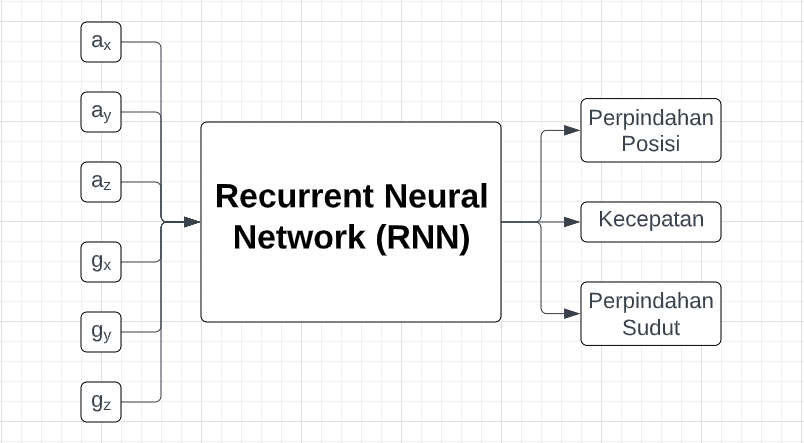
\includegraphics[scale=0.35]{gambar/RNN-3Dimensi.png}
  % Keterangan gambar yang diinputkan
  \caption{Pemrosesan data jarak yang ditempuh pada RNN}
  % Label referensi dari gambar yang diinputkan
  \label{fig:RNN-3D}
\end{figure}

Dengan menerapkan sistem \emph{Pose and Position} dalam dua dimensi (x,y) maka dari itu data yang dihasilkan pada nilai 3-Sumbu \emph{Gyroscope} 
yang memperoleh sumbu Az dan Gz tidak diperlukan karena jika dipakai, dibutuhkan setidaknya tiga dimensi (x,y,z) pada objek target.

% Contoh input gambar dengan format *.jpg
\begin{figure} [ht] \centering
  % Nama dari file gambar yang diinputkan
  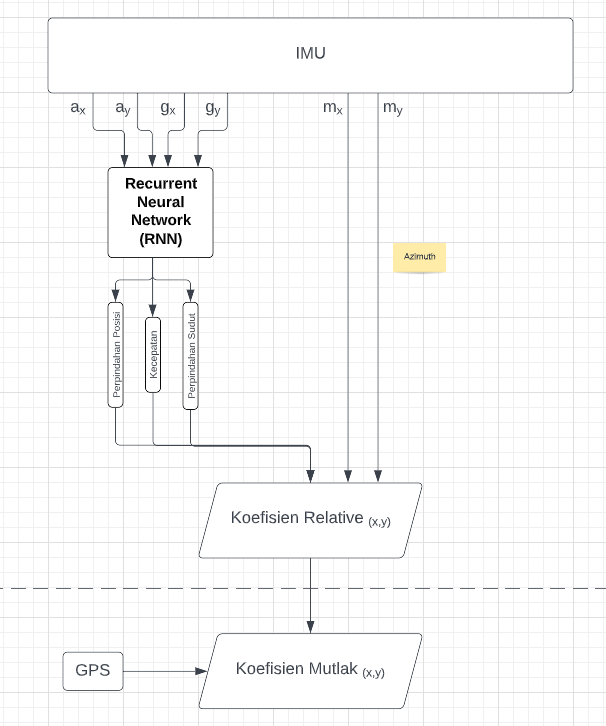
\includegraphics[scale=0.55]{gambar/IMU-to-KRel-KMut.png}
  % Keterangan gambar yang diinputkan
  \caption{Flowchart menentukan Koef. Relatif dengan RNN}
  % Label referensi dari gambar yang diinputkan
  \label{fig:Koef-Relatif}
\end{figure}

% Contoh penggunaan referensi dari gambar yang diinputkan
Pada \emph{flowchart} yang tertera di Gambar \ref{fig:Koef-Relatif} untuk mendapatkan posisi kendaraan memerlukan beberapa tahapan, mulai dari merangkai
seluruh alat-alat yang hendak digunakan untuk pengambilan data. Alat pengujian yang berupa mikrokontroller dengan sensor IMU dan beberapa komponen \emph{Electrical Wiring} 
akan dipasangkan pada kendaraan bermotor, Selanjutnya persiapkan dan instalasi beberapa \emph{Software} pendukung yang dibutuhkan dalam penelitian seperti,
kalibrasi sensor \emph{Inertial Measurement Unit} dengan \emph{Global Position System}, hingga instalasi mikrokontroller STM.  

\section{Bahan dan peralatan yang digunakan}

\subsection{Mikrokontroller STM32}
% Ubah paragraf berikut sesuai dengan Mikrokontroller STM32 dari tugas akhir
Mikrokontroler STM adalah rangkaian mikrokontroler yang dikembangkan dan diproduksi oleh STMicroelectronics, sebuah perusahaan semikonduktor global yang berbasis di Eropa. 
Mikrokontroler STM banyak digunakan dalam berbagai aplikasi termasuk elektronik konsumen, otomotif, kontrol industri, dan sistem komunikasi. Biasanya diprogram menggunakan 
bahasa pemrograman tingkat tinggi seperti C atau C++, dan dapat diprogram menggunakan berbagai alat pengembangan dan lingkungan pengembangan terintegrasi (IDE). 
Mikrokontroller ini juga menyediakan serangkaian pustaka dan alat perangkat lunak untuk membantu pengembang membuat aplikasi untuk mikrokontroler mereka. Seri STM32 didasarkan pada inti ARM Cortex-M3 yang dirancang khusus untuk aplikasi tertanam yang membutuhkan kinerja tinggi, biaya rendah, dan konsumsi daya rendah. Ini dibagi menjadi 
produk yang berbeda sesuai dengan arsitektur inti: Di antara mereka, seri STM32F meliputi: seri "ditingkatkan" STM32F103, seri "dasar" STM32F101, STM32F105, seri "interkoneksi" STM32F107, 
dan seri yang ditingkatkan dengan frekuensi clock 72MHz, yang merupakan produk kinerja tertinggi di antara produk serupa. 

% Contoh input gambar dengan format *.jpg
\begin{figure} [ht] \centering
  % Nama dari file gambar yang diinputkan
  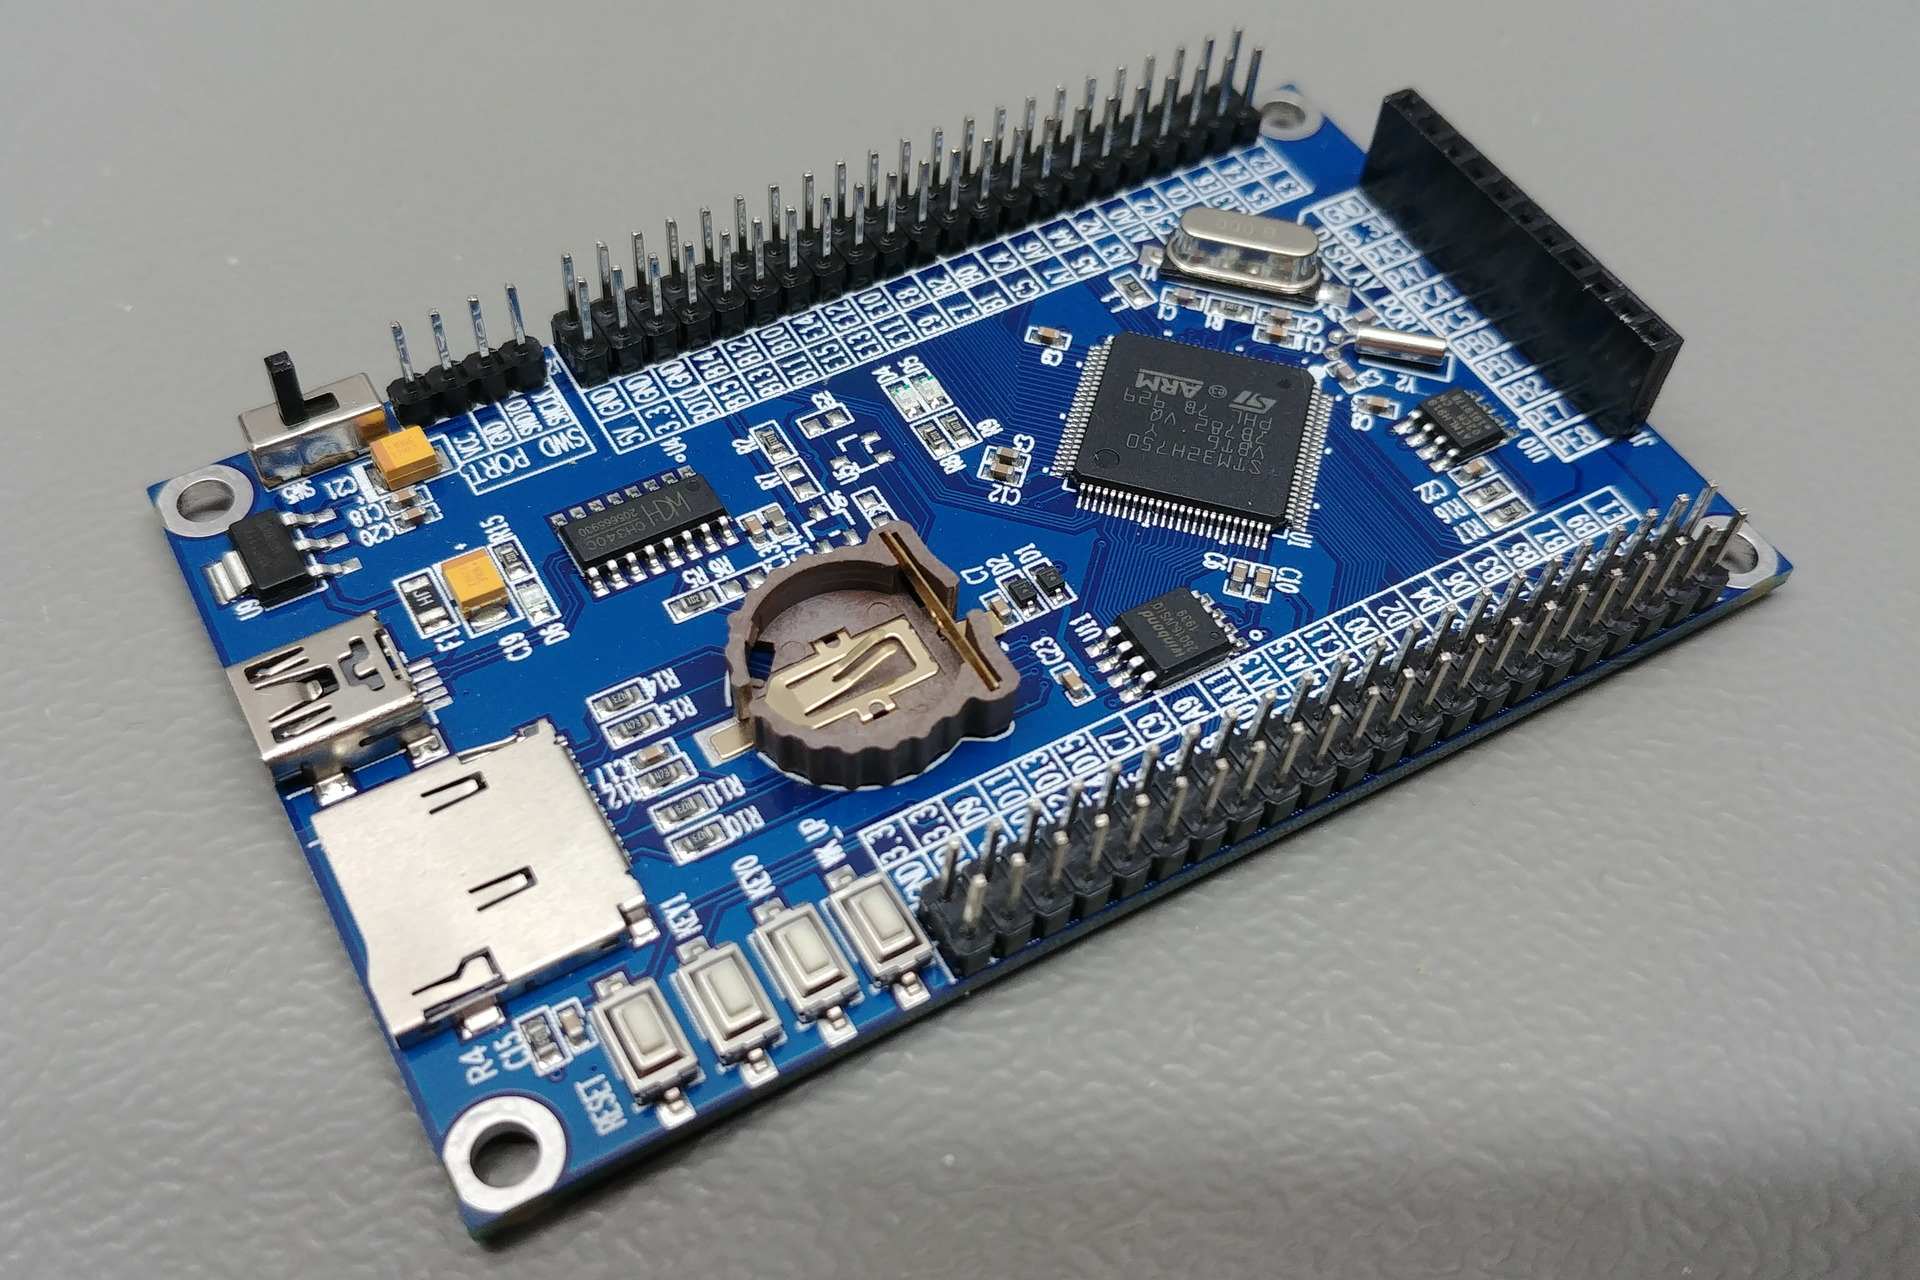
\includegraphics[scale=0.35]{gambar/STM32H750VBT6_Generic_Development_Board.jpg}
  % Keterangan gambar yang diinputkan
  \caption{ST-Microelectronics STM32H750VBT6, Arm Cortex-M7}
  % Label referensi dari gambar yang diinputkan
  \label{fig:STM-Board}
\end{figure}

\subsection{IMU Sensor Module MPU-9255}
% Ubah paragraf berikut sesuai dengan SENSOR MODULE IMU dari tugas akhir
MPU-9255 adalah \emph{Inertial Measurement Unit} (IMU) 9-sumbu yang dikembangkan oleh InvenSense, sebuah perusahaan yang berspesialisasi dalam desain dan pembuatan pelacakan gerak dan sensor 
pencitraan. MPU-9255 adalah perangkat kecil berdaya rendah yang dapat mengukur akselerasi, laju sudut, dan medan magnet dalam tiga dimensi. Ini umumnya digunakan dalam aplikasi seperti 
drone, robotika, realitas virtual, dan teknologi yang dapat dikenakan untuk memberikan informasi waktu nyata tentang orientasi, gerakan, dan akselerasi perangkat. 
Untuk menggunakan MPU-9255, Anda harus menghubungkannya ke mikrokontroler atau perangkat lain yang dapat berkomunikasi dengannya menggunakan antarmuka digital seperti I2C atau SPI. 
Nantinya kemudian perlu menulis kode untuk membaca data dari MPU-9255 dan menginterpretasikannya berdasarkan persyaratan aplikasi spesifik. InvenSense menyediakan serangkaian 
pustaka dan alat perangkat lunak untuk membantu pengembang membuat aplikasi menggunakan MPU-9255.

% Ubah paragraf berikut sesuai dengan PC/HP dari tugas akhir
\section{Urutan pelaksanaan penelitian}

% Ubah tabel berikut sesuai dengan isi dari rencana kerja
\newcommand{\w}{}
\newcommand{\G}{\cellcolor{gray}}
\begin{table}[h!]
  \begin{tabular}{|p{3.5cm}|c|c|c|c|c|c|c|c|c|c|c|c|c|c|c|c|}

    \hline
    \multirow{2}{*}{Kegiatan} & \multicolumn{16}{|c|}{Minggu} \\
    \cline{2-17} &
    1 & 2 & 3 & 4 & 5 & 6 & 7 & 8 & 9 & 10 & 11 & 12 & 13 & 14 & 15 & 16 \\
    \hline

    % Gunakan \G untuk mengisi sel dan \w untuk mengosongkan sel
    Studi pustaka &
    \G & \G & \G & \w & \w & \w & \w & \w & \w & \w & \w & \w & \w & \w & \w & \w \\
    \hline

    Perancangan alat dan Pengambilan data &
    \w & \G & \G & \G & \w & \w & \w & \w & \w & \w & \w & \w & \w & \w & \w & \w \\
    \hline

    Pengolahan data dan Pembuatan struktur model &
    \w & \w & \w & \w & \G & \G & \G & \G & \w & \w & \w & \w & \w & \w & \w & \w \\
    \hline

    Training, Validasi dan Pengujian Dataset &
    \w & \w & \w & \w & \w & \w & \G & \G & \G & \G & \w & \w & \w & \w & \w & \w \\
    \hline

    Penerapan model dan Penganalisaan hasil data &
    \w & \w & \w & \w & \w & \w & \w & \w & \G & \G & \G & \G & \w & \w & \w & \w \\
    \hline

    Perhitungan perbedaan K.Relatif (tanpa GPS) dengan K.Mutlak (dengan GPS) &
    \w & \w & \w & \w & \w & \w & \w & \w & \w & \w & \w & \w & \G & \G & \G & \w \\
    \hline

    Evaluasi penelitian &
    \w & \w & \w & \w & \w & \w & \w & \w & \w & \w & \w & \w & \w & \w & \G & \G \\
    \hline

    Penyusunan laporan &
    \G & \G & \G & \G & \G & \G & \G & \G & \G & \G & \G & \G & \G & \G & \G & \G \\
    \hline

  \end{tabular}
  \captionof{table}{Tabel timeline}
  \label{tbl:timeline}
\end{table}

Pada \emph{timeline} yang tertera di Tabel \ref{tbl:timeline}, terdapat 16 minggu pengerjaan penelitian, 
mulai dari satu bulan pertama ada Studi pustaka dengan Perancangan alat dan Pengambilan data, 
bertujuan untuk mengkaji ulang sedikit literatur yang kurang sesuai pada Proposal Tugas Akhir dan mulai 
merancang alat. dua bulan setelahnya adalah Pengolahan data dan Pembuatan model, serta Penerapan model dan 
Penganalisaan hasil data yang diperoleh. Di empat bulan terakhir adalah penambahan sedikit fitur atau mengetahui 
perbedaan antara dua buah obyek dengan substansi yang berbeda, jika ditemukan beberapa kesalahan dataset serta modeling 
bisa dilakukan evaluasi secara cepat.